\chapter{Discussion}
\label{sec:discussion}

This chapter includes a discussion about the gathered results.
Furthermore, the research questions introduced at the beginning of this work are addressed comprehensively and ultimately answered.
Therefore this chapter is divided into the individual research questions.

\subsubsection{1. What is the most effective vision-based approach for reliably identifying the rail track the train travels on, ensuring precise direction detection and robustness, especially in scenarios involving switches?}

In this work, the difference between rail track detection and rail track prediction is made in the introduction.
Rail track detection covers detecting all rails in an image, often with only one class, compared to rail track prediction, which distinguishes between the train track and other tracks.
Most state-of-the-art research only addresses rail track detection, not rail track prediction, often using semantic segmentation methods.
Only two papers found in the literature explore the topic of rail track prediction.
However, these papers proceed on the premise that the state of a switch cannot be determined.
They determine the train's track with complex post-processing algorithms, which cause a loss in speed.

To address the issue of identifying the state of the switches, such a system could be complemented with an object detection method.
Therefore, this study conducts experiments using models from the \ac{YOLO} series, which confirm the assumption, indicating the need for a fundamentally different approach.

This strategy is presented by \cite{tepNet2024}, the only project found in the literature that focuses on rail track prediction with the assumption of predicting switches correctly.
It changes the problem formulation to a regression problem and introduces a domain-specific loss function that considers positional error.
This approach shows promising results in terms of accuracy and real-time capability.
Therefore, this project presents the baseline for this work, and further experiments are conducted to increase the robustness of this system.

To answer the research question, even when there are still limitations to this method, it presents the most promising method in the state-of-the-art.
However, rail track prediction is an advancing research field, and systems need to be improved according to specific situations, like switch scenarios, to elevate the system to the maximum achievable level of accuracy and, consequently, safety.
This work presents techniques and approaches that prove to be more robust than the state-of-the-art ones.
However, more use case-specific research must be conducted when preparing the system for a real-world application.

\subsubsection{2. How can this application be implemented to run in real-time on an embedded device from the NVIDIA Jetson series?}

One goal of this work is to implement a real-time capable system.
All datasets in this work are some variations of RailSem19.
This dataset consists of images of YouTube videos primarily in 25 or 30 \ac{FPS}.
The temporal dataset also includes such videos.
Therefore, the system aims to speed up to 30 \ac{FPS}.
This results in a threshold for the latency of 33.33 ms or lower.
However, this is a simplified assumption based on available data rather than on a practical application.

When applied in an actual use case, the real-time capability primarily depends on the camera setup, the train velocity, the prediction, and the corresponding distances.
\autoref{fig:cameraSetup} shows a systematic camera setup with the most essential parameters, distances, and angles.
The green parts resemble the prediction with a length from the horizon line.

\autoref{func:RealTime} calculates the \ac{FPS} needed for a real-time capable system according to $d_{horizon}$ and $v_{train}$.
$d_{horizon}$ is defined by the geometry of the camera setup.
Theoretically, the system is still fast enough when the train travels a distance of $d_{horizon}$ between each frame.
That corresponds to a $\lambda$ of 1.
$\lambda$ is an additional parameter that defines how much the predicted area of the previous frame must overlap with the next frame.
$\lambda$ must be between 0 and 1.
The lower the value, the safer the system becomes.

\begin{figure}[H]
    \centering
    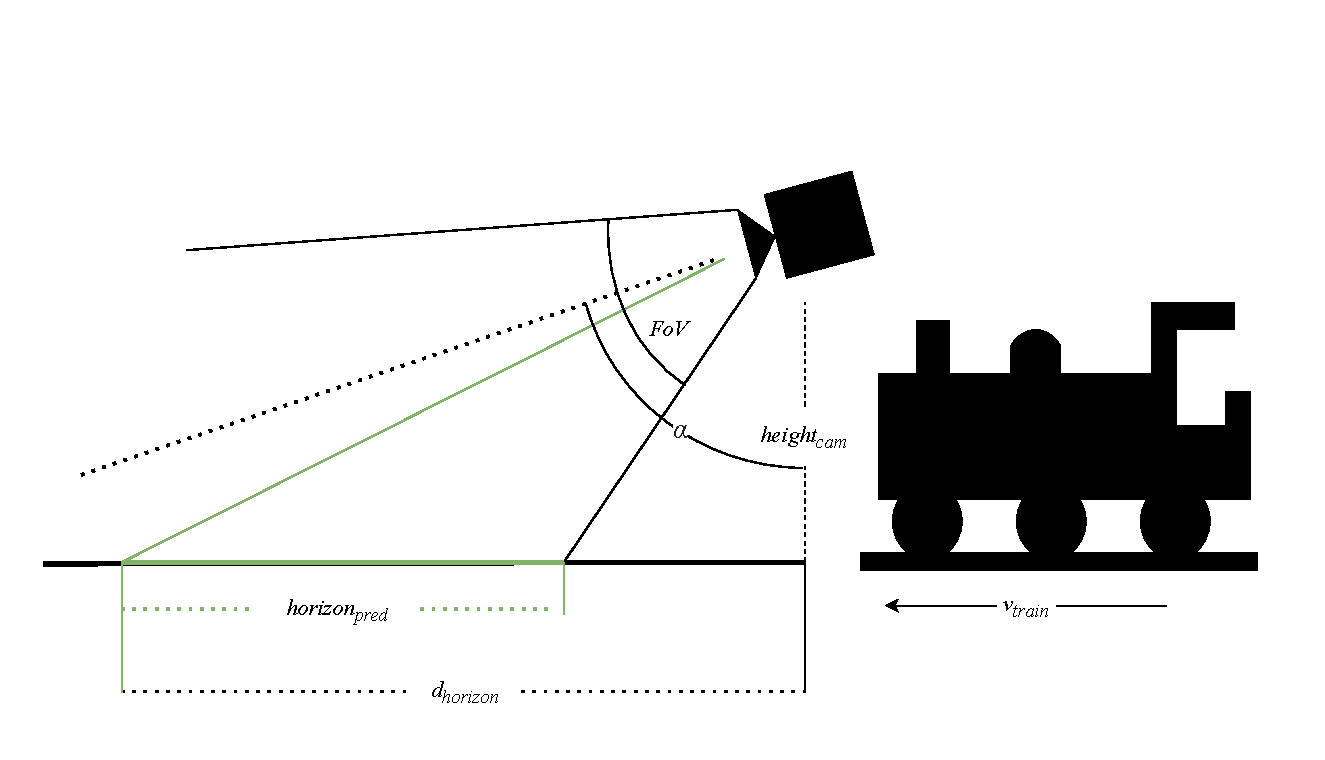
\includegraphics[width=0.8\textwidth]{PICs/discussion/Kameraaufbau.pdf}
    \caption{Camera setup}
    \label{fig:cameraSetup}
\end{figure}

\begin{align}
    FPS = \frac{v_{train}}{d_{horizon}} \times \frac{1}{\lambda}
    \label{func:RealTime}
\end{align}

\autoref{tab:variablesForRealTime} describes realistic values when the system is prepared for trains in Austria.
A GoPro Hero 10 \cite{goproHero10} is chosen because of its integrated mounting abilities and high $FoV$.
$\alpha$ and $height_{cam}$ are assumptions for Austrian trains.
$v_{train}$ is the fastest speed a train can drive in Austria \cite{geschwindigkeitZugAustria}.
Previous predictions like in \autoref{fig:autocropVideoComparison} lead to the assumption of $horizon_{pred}$.
480 pixels are roughly a third of the image that fits most predictions in this work.
\autoref{func:FPSValues} shows that only a speed of 5.1 \ac{FPS} is needed for a practical use case with the assumed parameters.
However, to increase safety, the overlap factor $\lambda$ is set to 0.17, which results in a frame rate of 30 \ac{FPS}.
Also interesting is that with this frame rate and the highest possible train speed, the distance traveled between frames is 2.45 m, as shown in \autoref{func:distanceBetweenFrameswith30FPS}.

\begin{table}[H]
    \centering
    \begin{tabular}{|l|c|c|}
    %\begin{tabular}{| p{0.3\linewidth} | p{0.6\linewidth} |}
        \hline
        \textbf{Parameters} & \textbf{Variables} & \textbf{Assumptions}\\
        \hline
        Camera model & & GoPro Hero 10 Black \cite{goproHero10} \\
        \hline
        Vertical Field of View & $FoV$ & $93^\circ$ \cite{goproHero10} \\
        \hline
        Camera mounting angle & $\alpha$ & $90^\circ$ \\
        \hline
        Camera mounting height & $height_{cam}$ & 4 m \\
        \hline
        Train speed & $v_{train}$ & 265 km/h \cite{geschwindigkeitZugAustria} $ \Leftrightarrow\ $ 73.61 m/s\\
        \hline
        Predicted horizon line & $ horizon_{pred} $ & 480 pixel from top \\
        \hline
        Overlap factor & $\lambda$ & 0.17 \\
        \hline
    \end{tabular}
    \caption{Variables for real-time calculation}
    \label{tab:variablesForRealTime}
\end{table}

\begin{align}
    d_{horizon} = \tan \left( \left( \frac{image_{height} - horizon_{pred}}{image_{height}} \times FoV \right) + \alpha - \frac{FoV}{2} \right) \times height_{cam}
    \label{func:dHorizon}
\end{align}

\begin{align}
    d_{horizon} = \tan \left( \left( \frac{720 - 480}{720} \times 93 \right) + 90 - \frac{93}{2} \right) \times 4 = 14.42 \, {m}
    \label{func:dHorizonValues}
\end{align}

\begin{align}
    FPS = \frac{v_{train}}{d_{horizon}} \times \frac{1}{\lambda} = \frac{73.61}{14.42} \times \frac{1}{1} = 5.1
    \label{func:FPSValues}
\end{align}

\begin{align}
    FPS = \frac{v_{train}}{d_{horizon}} \times \frac{1}{\lambda} = \frac{73.61}{14.42} \times \frac{1}{0.17} = 30
    \label{func:FPSValuesOverlap}
\end{align}

\begin{align}
    d_{frames} = \frac{v_{train}}{FPS} = \frac{73.61}{30} = 2.45 \, {m}
    \label{func:distanceBetweenFrameswith30FPS}
\end{align}

\vspace{1cm}

\begin{figure}[H]
    \centering
    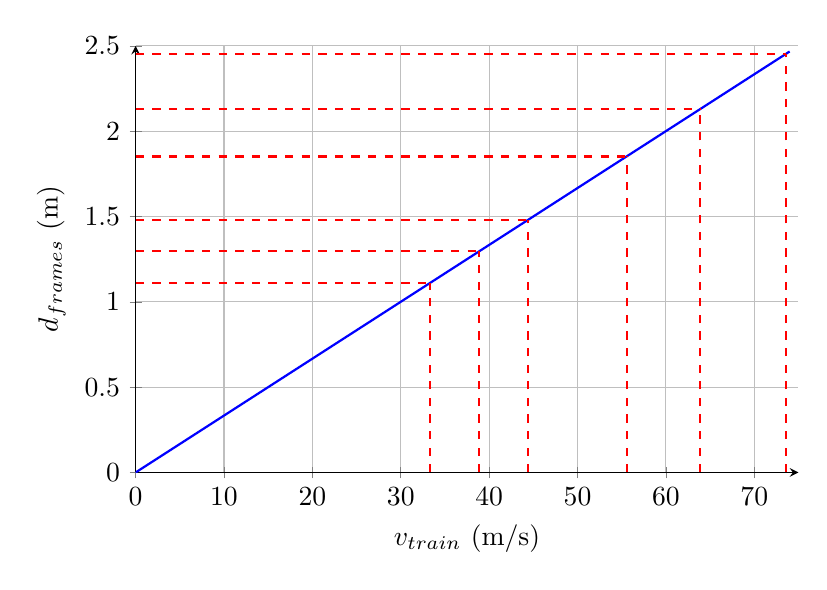
\begin{tikzpicture}
    \begin{axis}[
        width=10cm, height=7cm, % Größe des Graphen
        xlabel={$v_{train}$ (m/s)},
        ylabel={$d_{frames}$ (m)},
        xmin=0, xmax=75, % Begrenzung der x-Achse
        ymin=0, ymax=2.5, % Begrenzung der y-Achse
        grid=major,
        axis lines=left,
        legend style={at={(0.95,0.05)},anchor=south east},
        ]
        % Graph der Funktion y = 1/30 * x
        \addplot[blue, thick, domain=0:74, samples=100] {1/30 * x};
        
        % Vertikale und horizontale Linien für die gewünschten Geschwindigkeiten
        % 120 km/h = 33.33 m/s
        \draw[red, thick, dashed] (axis cs:33.33,0) -- (axis cs:33.33,1.111); % vertikal
        \draw[red, thick, dashed] (axis cs:0,1.111) -- (axis cs:33.33,1.111); % horizontal
        
        % 140 km/h = 38.89 m/s
        \draw[red, thick, dashed] (axis cs:38.89,0) -- (axis cs:38.89,1.2963); % vertikal
        \draw[red, thick, dashed] (axis cs:0,1.2963) -- (axis cs:38.89,1.2963); % horizontal
        
        % 160 km/h = 44.44 m/s
        \draw[red, thick, dashed] (axis cs:44.44,0) -- (axis cs:44.44,1.4813); % vertikal
        \draw[red, thick, dashed] (axis cs:0,1.4813) -- (axis cs:44.44,1.4813); % horizontal
        
        % 200 km/h = 55.56 m/s
        \draw[red, thick, dashed] (axis cs:55.56,0) -- (axis cs:55.56,1.8519); % vertikal
        \draw[red, thick, dashed] (axis cs:0,1.8519) -- (axis cs:55.56,1.8519); % horizontal
        
        % 230 km/h = 63.89 m/s
        \draw[red, thick, dashed] (axis cs:63.89,0) -- (axis cs:63.89,2.1297); % vertikal
        \draw[red, thick, dashed] (axis cs:0,2.1297) -- (axis cs:63.89,2.1297); % horizontal
        
        % 265 km/h = 73.61 m/s
        \draw[red, thick, dashed] (axis cs:73.61,0) -- (axis cs:73.61,2.4537); % vertikal
        \draw[red, thick, dashed] (axis cs:0,2.4537) -- (axis cs:73.61,2.4537); % horizontal
        
    \end{axis}
    \end{tikzpicture}
    \caption{Ratio between the train's speed and the distance it drives between frames with 30 \ac{FPS}. Red lines are the top speeds of all different trains from Austria: 120 km/h, 140 km/h, 160 km/h, 200 km/h, 230 km/h, 265 km/h, \cite{geschwindigkeitAllTrainsAustria}}
    \label{fig:ratioSpeedDistanceBetweenFrames}
\end{figure}

The following conclusions are drawn based on the calculated values required to assess a model's real-time capabilities.
Tables in \autoref{improvedTEPNetResults} show that almost every single-frame-based model achieves latencies below the threshold of 33.33 ms calculated from a frame rate of 30 \ac{FPS}.
The lightweight model architecture can explain this.
Only some versions of DenseNet exceed the desired target.

For answering this research question for the temporal models more factors must be considered.
\autoref{tab:temporalModelsResultsLatency} shows that the fastest temporal model is CNN\_FLAT\_FC in FP16.
Compared to the single-frame-based model, this method suffers from an increased latency, which is too high for inferring videos with 30 \ac{FPS}.
According to the calculations of \autoref{func:FPSValues}, the theoretical frame rate needed for real-time is 5.1 \ac{FPS}, which corresponds to a latency of 196.08 ms.
Since all temporal FP16 models have latencies below that, they are all theoretically real-time-capable.
FP32 models are too slow.

However, various methods could allow higher frame rates of input videos (30 \ac{FPS}) in practical operations.
Firstly, an increase in speed can be achieved by utilizing a MobileNet backbone.
\autoref{tab:temporalModelsResultsLatency} shows that this increases speed significantly and is within the limits of real-time capability when inferring 30 \ac{FPS} videos.
Secondly, when having a 30 \ac{FPS} video as input, only every third or fourth frame can be used.
This way the frame rate would effectively be reduced, increasing the allowed latency despite having a 30 \ac{FPS} video input.
An additional advantage of only inputting every third or fourth frame into the model is that the temporal context window increases even when the length of the sliding window remains the same.
Even though information between frames is lost, ten frames would cover a window of 30 or 40 frames.
Furthermore, using this technique decreases the number of frames in which the train is located directly over the switch, resulting in a smaller time frame that needs to be bridged.

In conclusion, temporal models can operate in real-time with a frame rate of 5.1 \ac{FPS}.
However, this presents an extreme case with an overlap factor of 1, which decreases the possible safety of the system.
That leads to the thought that the optimal trade-off must be found between the overlap of the predicted areas of consecutive frames and the frame rate.
Furthermore, in a practical application also the train's current speed can be incorporated which changes the real-time threshold and therefore frame rate adaptively.

\subsubsection{3. To what extent can the temporal dimension be leveraged to improve the accuracy of predictions in switch situations where the necessary information is no longer present in the current frame?}

\autoref{tab:temporalModelsResults} shows scenarios exist in which the original auto-crop is more advantageous than the adapted one, even though \autoref{sec:autocropResults} and \autoref{sec:qualitativeComparison} prove that the adapted one is more robust.
After analyzing models in these test cases, it becomes evident that the higher accuracy in \textbf{Switch 1} and \textbf{Switch 2} highly depends on the specific situations of these sequences.
\textbf{Switch 2} is a very complex situation with many steep angled switches present in the sequence, which is unusual for typical train infrastructure and only occurs in train stations or shunting yards.
Even the single-frame-based model is not designed for such situations and determines the direction of the train incorrectly in every frame.
\textbf{Switch 1}, on the other hand, is easy and is similar to a simple straight rail in which a single-frame-based model performs with high accuracy.
In this scenario, there is no need to improve performance with a temporal model.

The temporal component of the system is an approach to stabilize the single-frame-based model in switch scenarios.
However, temporal models also struggle when the scene is challenging, like \textbf{Switch 2}, and the single-frame-based model predicts 0/76 frames correctly when considering the direction.
When a scene is too easy, like \textbf{Switch 1} in which the single-frame-based model predicts 76/76 frames correctly concerning the direction, there is no need to try to stabilize the model with a temporal component.
The results of these two sequences lead to the thought that the created temporal dataset is not optimal and needs to be reviewed and changed.
In the fourth version of the dataset, questionable scenes like \textbf{Switch 1} and \textbf{Switch 2} can be removed since they do not represent typical train infrastructure or an inclusion is unnecessary.
Another approach could be to leave such scenes in the dataset but to gather more data so that these two scenes are no longer weighted so heavily in the evaluation.
However, since this process is very time-consuming, it is out of the scope of this work.
Additionally, the sequence length can be increased, and other scenarios can be included, like ones for trams, which is not the case until now.

Scenarios \textbf{Switch 3} and \textbf{Switch 4} prove that exploiting the temporal dimension makes a performance gain possible.
Single-frame-based models show typical problematic behaviors when driving over a switch in these two scenes.
Either the model chooses the wrong direction, experiences a drop in accuracy, and stabilizes after the switch, like in \textbf{Switch 4}.
This scenario is similar to the one visualized in \autoref{fig:limitationSwitch}.
Alternatively, the model fluctuates between the correct and wrong track, like in \textbf{Switch 3}.
Temporal models show a time-delayed drop in accuracy in cases like \textbf{Switch 4} and a more stable trend in \textbf{Switch 3}.
However, even though temporal models bring a performance gain at frames in which the train is located directly over a switch, single-frame-based models outperform temporal models in scenes without switches, according to the \ac{IoU}.
That is because single-frame-based models hit the rail pixels more precisely.

In conclusion, the temporal models can lead to a gain in accuracy.
\autoref{tab:temporalModelsResults} shows that when excluding questionable scenarios \textbf{Switch 1} and \textbf{Switch 2} an increase in \ac{IoU} accuracy of 15.25 \% compared to the adapted single-frame-based and an increase of 16.43 \% compared to the current state-of-the-art is possible.
Even when including these scenarios there is a gain in \ac{IoU} performance compared to the current state-of-the-art and the adapted model.
However, the results show that more research must be conducted for a temporal model to be applicable in a real-world scenario.
This is because, although the current state of this work achieves higher accuracy in switch cases, it comes at the expense of speed.
Furthermore, in scenarios without switches, single-frame-based models outperform temporal models, necessitating a method to potentially integrate both approaches and switch to the advantageous model for the given scenario.